
\subsection{Rhomencephalon: Myelencephalon}
\label{subsec:Myelencephalon} \index{Myelencephalon}
%%%%%%%%%%%%%%%%%%%%%%%%%%%%%%%%%%%%%%%%%%%%%%%%%%%%%%%%%%%
%%%%%%%%%%%%%%%%%%%%%%%%%%%%%%%%%%%%%%%%%%%%%%%%%%%%%%%%%%%

\subsubsection{Medulla} \index{Medulla oblongata}
%%%%%%%%%%%%%%%%%%%%%%%%%%%%%%%%%%%%%%%%%%%%%%%%%%%%%%%%%%%

Das Myelencephalon (Nachhirn) besteht aus der \textbf{Medulla oblongata}, auch verlängertes Rückenmark genannt. Sein 'Dach' ist dünn und weist kleine Falten auf \textsuperscript{\cite[Kap.~6]{storch2012lehrbuchzoo}}. Die Medulla liegt caudal des Pons und leitet zum Rückenmark über, dem es sowohl in Aufbau als auch Funktion ähnelt (Abb.~\ref{fig:medulla_schema},~\ref{fig:ruckenmark_schema}). Genau wie im Rückenmark sind die sensorischen Regionen dorsal im Hinterhorn (Flügelplatte) und die motorischen Regionen ventral im Vorderhorn (Grundplatte) in der grauen Substanz lokalisiert. Dabei liegen die somatosensorischen Regionen eher lateral und die viscerosensorischen Regionen eher medial. Im Vergleich zum Rückenmark ist der Zentralkanal erweitert und bildet den vierten Ventrikel. Beim Übergang von Rückenmark zur Medulla geht die dorso-ventrale Organisation des Rückenmarks in eine eher medio-laterale Organisation über \textsuperscript{\cite[Kap.~14]{penzlin2005tierphys}}.

\begin{figure}[H]
    \centering
    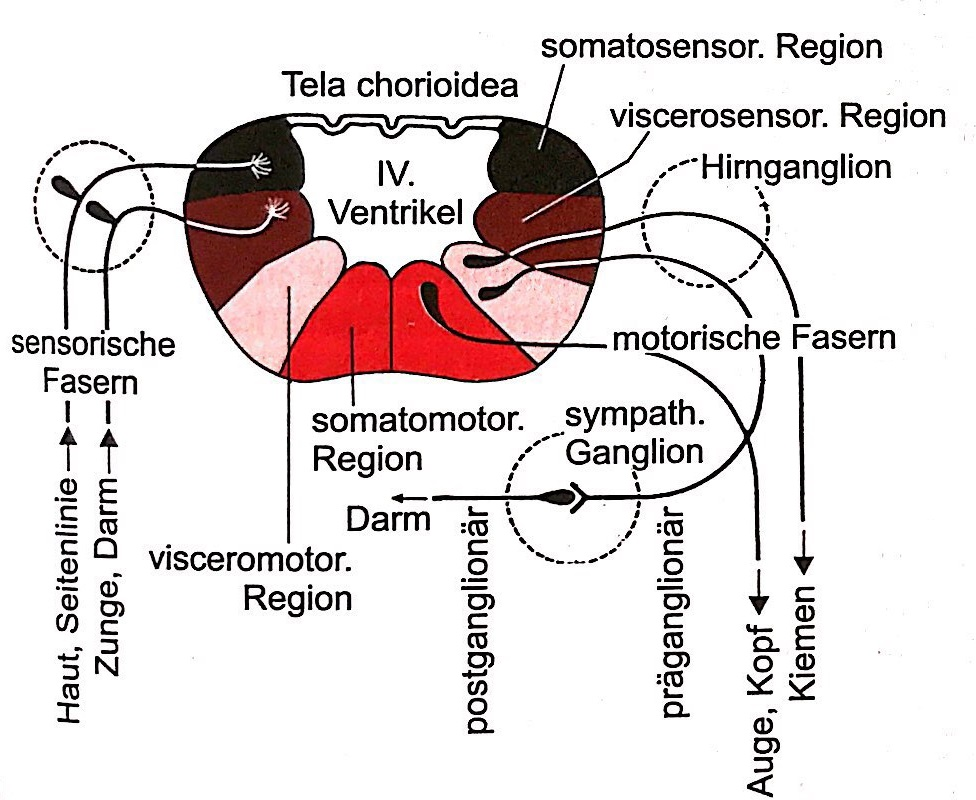
\includegraphics[width=0.6\textwidth]{pictures/Bilder_Jule/Andere/medulla_schema.jpg}
    \caption[Aufbau der Medulla]{\textbf{Aufbau der Medulla.} Gezeigt ist ein schematischer Querschnitt durch die Medulla, bzw. den Hirnstamm. Die superiore, bzw. dorsale, sensorische Seite ist nach oben, die inferiore, bzw. ventrale, motorische Seite nach unten orientiert.\\
    Abbildung aus \textit{Lehrbuch der Tierphysiologie}, Penzlin {\textsuperscript{\cite[Kap.~14]{penzlin2005tierphys}}}.}
    \label{fig:medulla_schema}
\end{figure}{}

\noindent Im Vergleich zu den anderen Hirnarealen entspringen der Medulla die meisten Hirnnerven (Abb.~\ref{fig:hirnnerven_schaf}). So liegen sowohl die primären sensorischen, als auch die primären motorischen Kerngebiete der Hirnnerven IV bis XII in der Medulla \textsuperscript{\cite[Kap.~14]{penzlin2005tierphys}}. Neben zahlreichen Hirnnervenkernen ist auch die \textbf{inferiore Olive}\index{Olive! untere Olive}, ein Kerngebiet, das in die Motorkontrolle involviert ist (Kap.~\ref{sec:Motorik})  \textsuperscript{\cite[Kap.~9]{crossman2014neuroanatomy}}, in der Medulla lokalisiert. Auch die Hinterstrangkerne, der \textbf{Nucleus cuneatus}\index{Nucleus! cuneatus} und der \textbf{Nucleus gracilis}\index{Nucleus! gracilis}, die Stationen der somatosensorischen Bahn darstellen (Kap.~\ref{subsubsec:tastsinn}) \textsuperscript{\cite[Kap.~5]{trepel2011neuroanatomie}} und der cochleare Nucleus\index{Nucleus! cochlearis}, sind in der Medulla lokalisiert (Abb.~\ref{fig:medulla_ratte}). Zusammen mit dem Pons\index{Pons} besteht die Funktion der Medulla unter anderem in der Regulation von Atmung und Kreislauf \textsuperscript{\cite[Kap.~14]{penzlin2005tierphys}}.

\begin{figure}[H]
    \centering
    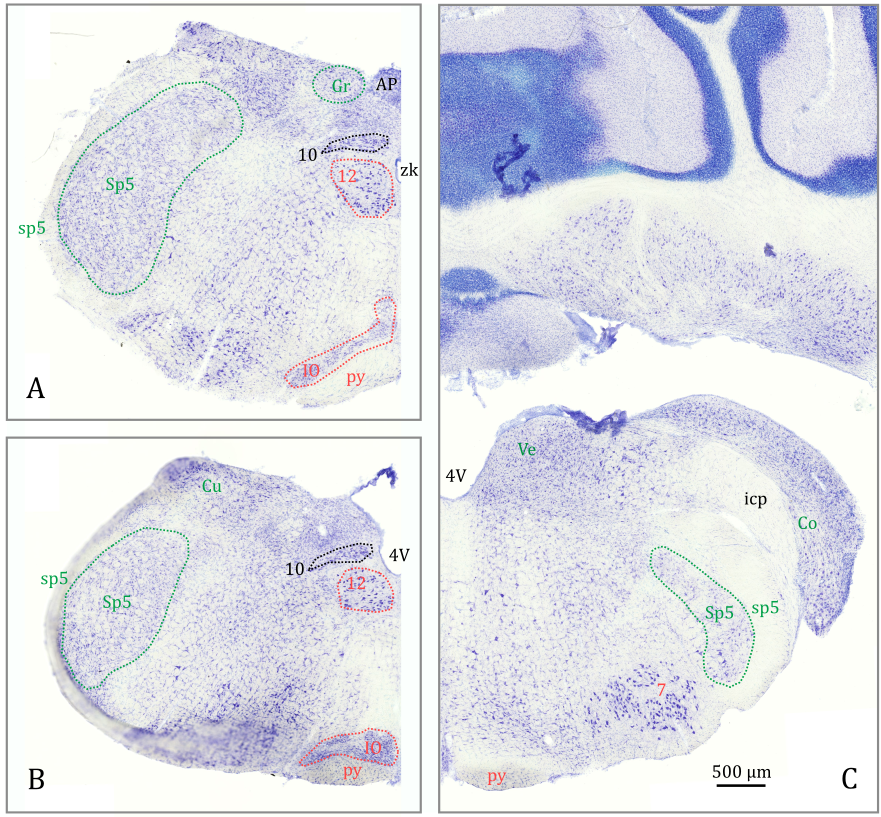
\includegraphics[width=\textwidth]{pictures/Bilder_Jule/Ratte/medulla.png}
    \caption[Medulla Ratte]{\textbf{Medulla Ratte.} Gezeigt sind Querschnitte durch die Medulla. \textbf{A} ist caudaler (N01-4), \textbf{B} rostraler (N02-4) lokalisiert. Auf \textbf{C}, dass sich weiter rostral befindet (N6-1), ist oben bereits das Cerebellum sichtbar. Sensorische Gebiete sind grün gekennzeichnet. Dazu gehören der Spinalkanal des N. trigeminus (sp5), sowie die zugehörigen Nuclei (Sp5), der Nucleus cochlearis (Co), der Nucleus vestibularis (Ve), sowie die Hinterstrangkerne: der Nucleus cuneatus (Cu) und der Nucleus gracilis (Gr). Motorische Gebiete sind rot markiert. Dazu gehören die Nuclei des N. hypoglossus (12), die Pyramidenbahn (py) und die inferiore Olive (IO). Ebenfalls gekennzeichnet sind die Nuclei des Vagus Nervs (10), der sowohl sensorische als auch motorische Funktionen besitzt, das Pedunculus cerebellaris inferior (icp), der Zentralkanal (zk) und der vierte Ventrikel (4V).} 
    \label{fig:medulla_ratte}
\end{figure}{}
